\documentclass[review]{elsarticle}
\usepackage{graphicx}
\usepackage{lmodern}
\usepackage{caption}
\usepackage{amsmath}
\usepackage{booktabs}

\usepackage{amsfonts}
\usepackage[T1]{fontenc}


% Bibliography: 
\usepackage{hyperref}
%\usepackage{natbib}
%\bibliographystyle{plainnat}


 
\usepackage{colortbl}
\usepackage[dvipsnames]{xcolor}

\usepackage{lineno,hyperref}
\modulolinenumbers[5]

\journal{Journal of \LaTeX\ Templates}

%%%%%%%%%%%%%%%%%%%%%%%
%% Elsevier bibliography styles
%%%%%%%%%%%%%%%%%%%%%%%
%% To change the style, put a % in front of the second line of the current style and
%% remove the % from the second line of the style you would like to use.
%%%%%%%%%%%%%%%%%%%%%%%

%% Numbered
%\bibliographystyle{model1-num-names}

%% Numbered without titles
%\bibliographystyle{model1a-num-names}

%% Harvard
%\bibliographystyle{model2-names.bst}\biboptions{authoryear}

%% Vancouver numbered
%\usepackage{numcompress}\bibliographystyle{model3-num-names}

%% Vancouver name/year
%\usepackage{numcompress}\bibliographystyle{model4-names}\biboptions{authoryear}

%% APA style
%\bibliographystyle{model5-names}\biboptions{authoryear}

%% AMA style
%\usepackage{numcompress}\bibliographystyle{model6-num-names}

%% `Elsevier LaTeX' style
\bibliographystyle{elsarticle-num}
%%%%%%%%%%%%%%%%%%%%%%%

\begin{document}

\begin{frontmatter}

\title{Multi-SpaM: a Maximum-Likelihood approach to Phylogeny Reconstruction based on Multiple Spaced-Word Matches}
\tnotetext[mytitlenote]{Fully documented templates are available in the elsarticle package on \href{http://www.ctan.org/tex-archive/macros/latex/contrib/elsarticle}{CTAN}.}

%% Group authors per affiliation:
\author{Md. Nazmul Hasan }
\ead{0419052003}
\ead{nazmulcse25@gmail.com}

%% or include affiliations in footnotes:
\author{Arefin Rahman Niloy}
\ead{108052108}
\ead{arefinniloy@gmail.com}
\end{frontmatter}

\begin{abstract}
\textbf{Motivation:} 
Word-based or `alignment-free' methods for phylogeny
reconstruction are much faster
than traditional approaches, but they are generally less
accurate. Most of these methods calculate pairwise distances for a set
of input sequences, for example from {\em word frequencies}, from so-called {\em spaced-word matches} or from the average {\em length of common substrings}.
\\ 
\textbf{Results:}
In this paper, we propose the first word-based approach to tree reconstruction that is based on multiple sequence comparison and {\em Maximum Likelihood}.
Our algorithm first samples small, gap-free
alignments involving four taxa each. For each of these alignments,
it then calculates a quartet tree and, finally, the program {\em Quartet MaxCut} is used to infer a super tree topology for the full set of input
taxa from the calculated quartet trees. Experimental results show that trees
calculated with our approach are of high quality.
%

\end{abstract}


\section{Introduction}


To gain a better understanding of the evolution of genes or species, reconstructing accurate phylogenetic trees is essential. This can be done using standard methods which rely on  \textit{sequence alignments}, either of entire genomes or of sets of orthologous genes or proteins.    
\textit{Character-based} methods such as {\em Maximum Parsimony} \cite{far:70,fit:71} or {\em Maximum Likelihood} \cite{fel:81} infer trees based on evolutionary substitution events that 
%are indicated by the alignment to 
may have happened since the species evolved from a common ancestor. 
These methods are generally considered to be  accurate, 
as long as the underlying alignments are of high quality, {and as long
as suitable substitution models are used}. However,
for the task of multiple alignment no exact polynomial-time algorithm 
exists, and even heuristic approaches can be time consuming~\cite{sie:wil:din:etal:11}. 
Moreover, 
the most popular heuristic for multiple alignment, the {\em progressive
alignment} \cite{fen:doo:87}, has been shown to be relatively unstable: 
multiple alignments calculated with  
progressive approaches and trees inferred from these alignments  
depend on the underlying {\em guide trees} and even on the
order of the input sequences \cite{cha:flo:tom:etal:18}.
In addition to these difficulties, 
exact algorithms for {character-based} phylogeny approaches  
are themselves 
{\em NP hard}~\cite{cho:tul:05,AAM:FouldsG1982}.

{\em Distance} methods, by contrast, {infer phylogenies by estimating}  evolutionary distances for all pairs of input taxa \cite{fel:84}. Here,  
 pairwise alignments are sufficient which can be faster calculated than multiple alignments, but still require runtime proportional to the product of the lengths of the aligned sequences. There is a loss in accuracy, however, compared to character-based approaches, as all of the information about evolutionary events is reduced to a single number for each pair of taxa, 
and not more than two sequences are considered simultaneously, as opposed to character-based approaches, where all sequences are examined simultaneously. 
%In particular, different substitution rates in some areas of the genomes cannot be factored in this way.
%
% The final trees are obtained by hierarchical clustering according to the distance matrices, most commonly with  
%
The final trees 
%
 are obtained by clustering based on distance matrices, most commonly with \textit{Neighbor Joining}~\cite{sai:nei:87}.
Since both pairwise and multiple sequence alignments are computationally expensive, they are ill-suited for the increasingly large datasets that are available today due to the next generation sequencing techniques. 


In recent years, a number of \textit{alignment-free} approaches to genome-based phylogeny reconstruction have been published which are very fast in comparison to alignment-based methods~\cite{son:ren:rei:etal:14,zie:vin:alm:kar:17,ber:cha:rag:16,bro:gri:otw:16,piz:16,ren:bai:you:etal:18}. 
Another advantage of these new methods is that they circumvent some  well-known problems in genome alignment such as genome rearrangements and duplications. Moreover, alignment-free methods can be applied 
to incomplete sequence sets and even to collections of unassembled reads \cite{roy:vis:bha:13,son:ren:zha:etal:13,yi:jin:13,com:sch:14}.
 A disadvantage of these methods is that they are, in general, considerably less accurate than slower, alignment-based methods. 

% match lengths methods like cophylog andi kmacs

Some `alignment-free' approaches compare fixed-length {\em words} of the input sequences to each other, so   
-- despite being called `alignment-free' -- they are using local pairwise `mini-alignments'.  
Recently, methods have been proposed that estimate phylogenetic distances based on the relative frequency of mismatches in such local alignments.  
An example is \textit{co-phylog}~\cite{yi:jin:13} which finds short gap-free alignments of a fixed length, consisting of matching nucleotide pairs only, except for the middle position where a mismatch is allowed.  
%Taking all of these alignments for a pair of sequences, 
Phylogenetic distances are estimated from the fraction of such alignments for which the middle position is a mismatch. As a generalization of this approach, \textit{andi}~\cite{hau:klo:pfa:14} uses pairs of maximal exact word matches that have the same distance to each other in both sequences; the frequency  of mismatches in the segments between those matches is then used to  estimate the number of substitutions per position between two input sequences. 

{\em co-phylog} and {\em andi} require a minimum length of the flanking word matches in order to reduce the number of random background matches. Threfore, they tend not to perform well on distantly related sequences where long exact matches are less frequent. 
%
Moreover, the number of random segment matches grows quadratically with the length of the input sequences while the expected number of homologous matches grows only linearly. Thus, longer exact matches are necessary in these approaches to limit the number of background matches if longer sequences are compared. This, in turn, reduces the number of {homologies} that are found, and therefore the amount of information that can be used to calculate accurate distances.
%
Other alignment-free approaches are based on the length of maximal common substrings between sequences. These approaches are also very efficient, since  common substrings can be rapidly found using suffix trees or related data structures \cite{uli:bur:tul:cho:06,hau:pfa:dom:wie:09}.  As a generalization of this approach, some methods use longest common substrings with a certain number of mismatches \cite{lei:mor:14,tha:apo:alu:16,tha:cho:liu:etal:17,mor:sch:lei:17,aya:cha:ili:pis:18}. 


Recently, we proposed to use words with {\em wildcard characters} -- so-called \textit{spaced words} -- for alignment-free sequence comparison \cite{lei:bod:hor:lin:mor:14,hor:lin:bod:etal:14}. 
Here, a  binary pattern of {\em match} and {\em don't-care} positions specifies the positions of the {\em wildcard} characters \cite{oun:lon:15,noe:17,gir:com:piz:18}. In \textit{Filtered Spaced-Word Matches (FSWM)}~\cite{lei:soh:mor:17} and {\em Proteome-based Spaced-word Matches (Prot-SpaM)} \cite{lei:sch:sch:etal:18}, alignments of such spaced words are used, where sequence positions must match at the {\em match} positions while mismatches are allowed at the \textit{don't care positions}. 
A score is calculated for every such spaced-word match in order to remove -- or {\em filter out} -- {\em background} spaced-word matches; the mismatch frequency of the remaining \textit{homologous} spaced-word matches is then used to estimate the number of substitutions per position that happened since two sequences evolved from their last common ancestor. The filtering step allows us to use patterns with fewer match positions in comparison to above mentioned methods {\em co-phylog} and {\em andi}, since the vast majority of the background noise can be eliminated reliably by looking at the {\em don't-care} positions of the initially found spaced-word matches. As a result, the phylogenetic distances calculated by {\em FSMW} and {\em Prot-SpaM} are generally rather accurate, even for large and distantly related sequences.




In this paper, we introduce a novel approach to phylogeny reconstruction called {\em \underline{\smash{Multi}}ple \underline{\smash{Spa}}ced-Word \underline{\smash{M}}atches (Multi-SpaM)} that combines the {\em speed} of the so-called `alignment-free' methods with the 
{\em accuracy} of the  {\em Maximum-Likelihood} approach. While other alignment-free methods are limited to {\em pairwise} sequence comparison, we generalize the above outlined {{\em spaced-word} approach to {\em multiple} sequence comparison. For a binary pattern of {\em match} and {\em don't care} positions, {\em Multi-SpaM} identifies {\em quartet blocks} of four matching spaced words each, {\em i.e.} gap-free four-way alignments with matching nucleotides at the {\em match} positions of the underlying  binary pattern and possible mismatches at the {\em don't care} positions, see Figure~\ref{fig:block} for an example. 
% For each such quartet block, an optimal tree topology is calculated with the {\em Maximum-Likelihood} software {\em RAxML}~\cite{sta:14}.
For each such quartet block, an optimal {\em Maximum-Likelihood} tree topology is calculated with the software {\em RAxML}~\cite{sta:14}.
The \textit{Quartet MaxCut} algorithm~\cite{sni:rao:12} is then used to combine the calculated quartet tree topologies into a super tree. 
%
We show that on both simulated and real data, {\em Multi-SpaM} produces phylogenetic trees of high quality and often outperforms other alignment-free methods.  
%A preliminary version of the present paper has been uploaded to the preprint server {\em arXiv} \cite{den:lei:mor:18}. 


\section{Material and Method}

To describe our method, we first need some formal definitions. A \textit{spaced word} of length~$\ell$ exists in the context of a binary pattern $P \in \{0,1\}^\ell$ of the same length. This pattern marks every position as either a \textit{match position} in case of a 1 or as a \textit{don't care position} in case of a 0. The number of match positions is called the \textit{weight} of the pattern.
Given such a pattern~$P$, a \textit{spaced word}~$w$ is a word of length~$\ell$ over the alphabet \{A,C,G,T,*\} such that $w(i) = *$ if and only if $P(i) = 0$, {\em i.e.} if and only if $i$ is a {\em don't care} position. The symbol `$*$' is interpreted as a  `wildcard' character. 
%
For a DNA Sequence $S$ of length $n$ and a position $0 \leq i \leq n-l+1$, we say that a \textit{spaced word} $w$ occurs in $S$ at position~$i$ -- or that  $[S,i]$ is an {\em occurrence} of $w$ -- if $S(i + j) = w(j)$ for all match positions~$j$.
%\begin{equation*}
% w(j) = \begin{cases}
% S(i + j) & $if $j$ is a match position$ \\
% * & $if $j$ is a don't care position$ \\
% \end{cases}
%\end{equation*}
%for $0 \leq j \leq l - 1$. 
This follows the definition that we previously used \cite{lei:bod:hor:lin:mor:14,mor:zhu:hor:lei:15}.

A pair $\left([S,i],[S',i']\right)$ of occurrences of the same spaced word~$w$ is called a {\em spaced-word match}. For a substitution matrix assigning a {\em score}$s( X,Y)$ to every pair $(X,Y)$ of nucleotides, we define the {\em score} of a spaced word match $([S,i],[S',i'])$ as  
$$\sum_{P(k) = 0}  s( S(i+k),S'(i'+k))$$
That is, if we align the two occurrences of $w$ to each other, the score of the spaced-word match is the sum of the scores of the nucleotides aligned to each other at the {\em don't-care} positions of~$P$. In {\em Multi-SpaM}, we are using the  nucleotide substitution matrix below that has been proposed by
Chiaromonte {\em et al.}~\cite{chi:yap:mil:02}:

\[
\begin{array}{crrrr}
  & A  &   C  &  G  &   T  \\
A & 91 & -114 & -31 & -123 \\
C &    & 100  &-125 &  -31 \\
G &    &      & 100 & -114 \\
T &    &      &     &   91 \\
\end{array}
\]

{\em Multi-SpaM} starts with generating a binary pattern~$P$ with  user-defined length~$\ell$ and weight~$w$. By default, we use values $\ell=110$ and $w=10$, {\em i.e.} by default the pattern has 10 {\em match positions} and 100 {\em don't-care} positions, but other values for $\ell$ and $w$ can be chosen by the user. Given these parameters, $P$ is calculated by running our previously developed software tool {\em rasbhari}~\cite{hah:lei:oun:etal:16}.  

As a basis for phylogeny reconstruction, we are using four-way alignments consisting of occurrences of the same spaced word with respect to $P$ in four different sequences. We call such an alignment a {\em quartet $P$-block} or a $P$-{\em block}, for short. A $P$-block is thus a gap-free alignment of length $\ell$ where in the $k$-th column identical nucleotides are aligned if $k$ is a {\em  match} position in $P$, while mismatches are possible if $k$ is a {\em don't-care} position, see Figure~\ref{fig:block} for an example.   
%
%
%
Note that the number of such $P$-blocks can be very large: if there are $n$ occurrences of a spaced-word~$w$ in $n$ different sequences, then this gives rise to $n \choose 4$ different $P$-blocks. 
Thus, instead of using all possible $P$-blocks, {\em Multi-SpaM} randomly samples a limited number of $P$-blocks  to keep the program runtime under control.  

Moreover, for phylogeny reconstruction, we want to use $P$-blocks that are likely to represent true homologies. Therefore, we introduce the following definition: a $P$-block -- {\em i.e.} a set of four occurrences of the same spaced word~$w$ --  is called a {\em homologous $P$-block} if it contains at least {\em one} occurrence $[S_i,p]$ of $w$  such that all remaining three occurrences of $w$  have positive scores when compared to $[S_i,p]$.  
%
To sample a list of homologous $P$-blocks, we randomly select spaced-word occurrences with respect to~$P$ from the input sequences and their reverse complements. For each selected $[S_i,p]$, we then randomly select occurrences of the same spaced word from sequences $S_j \not= S_i$, until we have found three occurrences of $w$ from three different sequences that all have positive scores with $[S_i,p]$.
%


%




% In the above described procedure, 
To find spaced-word matches efficiently  we
first sort the list of all occurrences of spaced words with respect to $P$ in lexicographic order. This way, we obtain a list of spaced-word occurrences where all occurrences of the same spaced word $w$ are appearing as a contiguous block. 
Once we have sampled a homologous $P$-block as described, we remove the four occurrences of $w$ from our list of spaced-word occurrences, so no two of the sampled $P$-blocks can contain the same occurrence of a spaced word. 
%
The algorithm continues to sample $P$-blocks until no further $P$-blocks can be found, or until a given number 
of  $P$-blocks is reached. By default, {\em Multi-SpaM} uses a maximal number of $M=1,000,000$ $P$-blocks, but this parameter can be adjusted by the user.  


{For each of the sampled quartet $P$-blocks, we infer an unrooted tree topology. This most basic {\em unrooted} phylogenetic unit is called a \textit{quartet} topology; there are three possible different quartet
topologies for a set of four taxa.  
To identify the best of these three topologies, we use the {\em Maximum Likelihood} program {\em RAxML}~\cite{sta:14}.  We note that 
{\em RAxML} is a general {\em Maximum-Likelihood} software, its use in our context is fairly degenerated, as we only use it to 
infer optimal quartet topologies.}\\
%
\begin{figure}[h]
\centering
%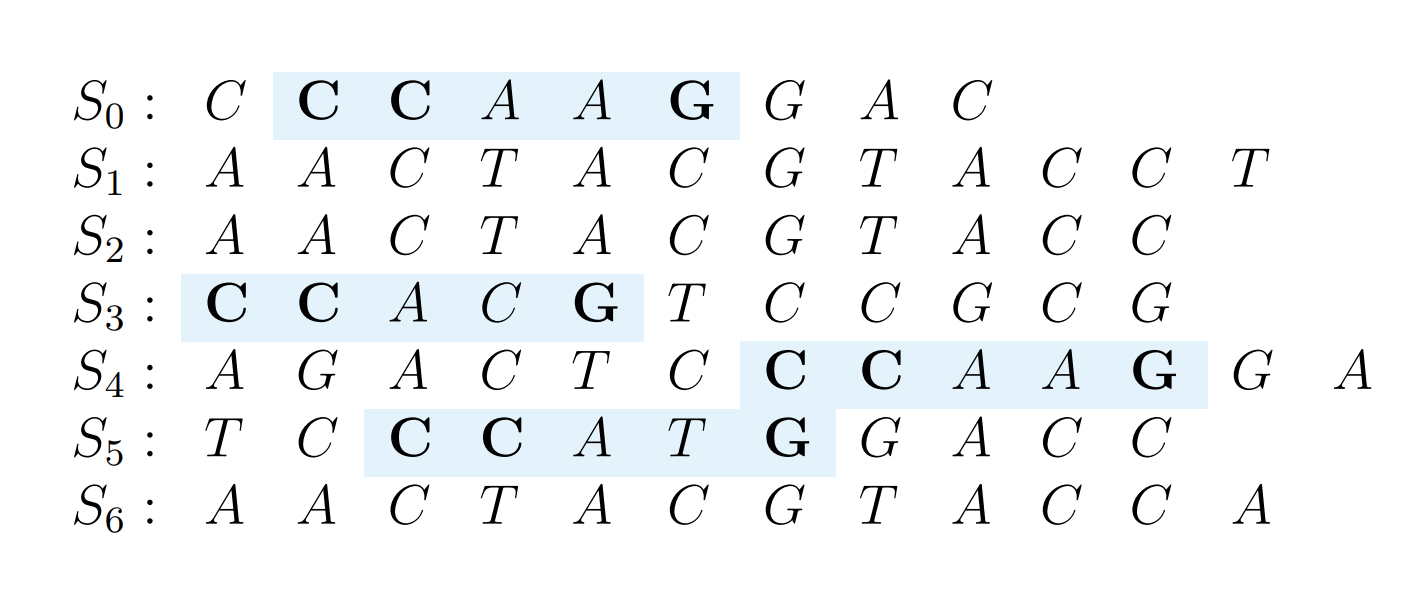
\includegraphics[width=0.5\linewidth]{\fig/quartet_tree}
\label{fig:qrtt}
\caption{Example of a quartet tree topology.}
\end{figure}

After having the optimal tree topology for each of the sampled quartet P-blocks, we need to amalgamate  them into a single tree spanning the entire taxa set. This task is denoted the {\em Supertree Task}~\cite{bininda-book-2004}
and is known to be {\em NP hard}, even for the special case where the input 
is limited to 
quartets topologies, as in our case~\cite{NPsteel}. Nevertheless there are several heuristics
for this task, with {\em MRP}~\cite{Baum1992,Ragan1992} the most popular. Here we chose to use {\em Quartet MaxCut}~\cite{sni:rao:10,sni:rao:12}
that proved to be faster and more accurate for this kind of input~\cite{Avni-JME-2018}. In brief, {\em Quartet MaxCut} partitions recursively the taxa set where
each such partition corresponds to a split in the final tree. In each
such recursive step, a graph over the taxa set is built where the set
of quartets induces the edge set in that graph. The idea is to
partition the vertex set (the taxa) such that the minimum quartets are
violated. This is achieved by a {\em semidefinite-programming}-like
algorithm that embeds the graph on the unit sphere and applies a
random hyperplane through the sphere.



\begin{itemize}
\item document style
\item baselineskip
\item front matter
\item keywords and MSC codes
\item theorems, definitions and proofs
\item lables of enumerations
\item citation style and labeling.
\end{itemize}

\section{Front matter}

The author names and affiliations could be formatted in two ways:
\begin{enumerate}[(1)]
\item Group the authors per affiliation.
\item Use footnotes to indicate the affiliations.
\end{enumerate}
See the front matter of this document for examples. You are recommended to conform your choice to the journal you are submitting to.

\section{Bibliography styles}

There are various bibliography styles available. You can select the style of your choice in the preamble of this document. These styles are Elsevier styles based on standard styles like Harvard and Vancouver. Please use Bib\TeX\ to generate your bibliography and include DOIs whenever available.

Here are two sample references: \cite{Feynman1963118,Dirac1953888}.

\section*{References}

\begin{thebibliography}{10}

\bibitem{ang:sal:11}
Samuel~V. Angiuoli and Steven~L. Salzberg.
\newblock Mugsy: fast multiple alignment of closely related whole genomes.
\newblock {\em Bioinformatics}, 27:334--342, 2011.

\bibitem{Avni-JME-2018}
Eliran Avni, Zahi Yona, Reuven Cohen, and Sagi Snir.
\newblock The performance of two supertree schemes compared using synthetic and
  real data quartet input.
\newblock {\em Journal of Molecular Evolution}, 86:150--165, 2018.

\bibitem{aya:cha:ili:pis:18}
Lorraine~A.K. Ayad, Panagiotis Charalampopoulos, Costas~S. Iliopoulos, and
  Solon~P. Pissis.
\newblock Longest common prefixes with $k$-errors and applications.
\newblock {\em arXiv:1801.04425 [cs.DS]}, 2018.

\bibitem{Baum1992}
B.R. Baum.
\newblock Combining trees as a way of combining data sets for phylogenetic
  inference.
\newblock {\em Taxon}, 41:3--10, 1992.

\bibitem{ber:cha:rag:16}
Guillaume Bernard, Cheong~Xin Chan, and Mark~A Ragan.
\newblock Alignment-free microbial phylogenomics under scenarios of sequence
  divergence, genome rearrangement and lateral genetic transfer.
\newblock {\em Scientific Reports}, 6:28970, 2016.

\bibitem{bininda-book-2004}
O.R.P. Bininda-Emonds.
\newblock {\em Phylogenetic supertrees: Combining information to reveal the
  Tree of Life}.
\newblock Computational Biology. Springer, 2004.

\bibitem{bro:gri:otw:16}
Raquel Bromberg, Nick~V. Grishin, and Zbyszek Otwinowski.
\newblock Phylogeny reconstruction with alignment-free method that corrects for
  horizontal gene transfer.
\newblock {\em PLOS Comput Biol}, 12:e1004985, 2016.

\bibitem{cat:pet:gia:ros:17}
Giuseppe Cattaneo, Umberto Ferraro~Petrillo, Raffaele Giancarlo, and Gianluca
  Roscigno.
\newblock An effective extension of the applicability of alignment-free
  biological sequence comparison algorithms with {H}adoop.
\newblock {\em The Journal of Supercomputing}, 73:1467--1483, 2017.

\bibitem{cha:flo:tom:etal:18}
Maria Chatzou, Evan~W. Floden, Paolo Di~Tommaso, Olivier Gascuel, and Cedric
  Notredame.
\newblock Generalized bootstrap supports for phylogenetic analyses of protein
  sequences incorporating alignment uncertainty.
\newblock {\em Systematic Biology}, page syx096, 2018.

\bibitem{chi:yap:mil:02}
Francesca Chiaromonte, Von~Bing Yap, and Webb Miller.
\newblock Scoring pairwise genomic sequence alignments.
\newblock In Russ~B. Altman, A.~Keith Dunker, Lawrence Hunter, and Teri~E.
  Klein, editors, {\em Pacific Symposium on Biocomputing}, pages 115--126,
  2002.

\bibitem{cho:tul:05}
Benny Chor and Tamir Tuller.
\newblock Maximum likelihood of evolutionary trees is hard.
\newblock In Satoru Miyano, Jill Mesirov, Simon Kasif, Sorin Istrail, Pavel~A.
  Pevzner, and Michael Waterman, editors, {\em Research in Computational
  Molecular Biology}, pages 296--310, Berlin, Heidelberg, 2005. Springer Berlin
  Heidelberg.

\bibitem{com:sch:14}
Matteo Comin and Michele Schimd.
\newblock Assembly-free genome comparison based on next-generation sequencing
  reads and variable length patterns.
\newblock {\em BMC Bioinformatics}, 15:S1, 2014.

\bibitem{dal:ani:gon:des:12}
Daniel~A. Dalquen, Maria Anisimova, Gaston~H. Gonnet, and Christophe Dessimoz.
\newblock {ALF} - a simulation framework for genome evolution.
\newblock {\em Molecular Biology and Evolution}, 29:1115--1123, 2012.

\bibitem{far:70}
James~S. Farris.
\newblock Methods for computing wagner trees.
\newblock {\em Systematic Biology}, 19:83--92, 1970.

\bibitem{fel:81}
Joseph Felsenstein.
\newblock Evolutionary trees from {DNA} sequences:a maximum likelihood
  approach.
\newblock {\em Journal of Molecular Evolution}, 17:368--376, 1981.

\bibitem{fel:84}
Joseph Felsenstein.
\newblock Distance methods for inferring phylogenies: a justification.
\newblock {\em Evolution; international journal of organic evolution},
  38:16--24, 1984.

\bibitem{fel:89}
Joseph Felsenstein.
\newblock {PHYLIP - Phylogeny Inference Package (Version 3.2)}.
\newblock {\em Cladistics}, 5:164--166, 1989.

\bibitem{fel:04}
Joseph Felsenstein.
\newblock {\em Inferring Phylogenies}.
\newblock Sinauer Associates, Sunderland, MA, USA, 2004.

\bibitem{fen:doo:87}
D.~F. Feng and R.~F. Doolittle.
\newblock Progressive sequence alignment as a prerequisite to correct
  phylogenetic trees.
\newblock {\em J. Mol. Evol.}, 25:351--360, 1987.

\bibitem{fit:71}
Walter Fitch.
\newblock Toward defining the course of evolution: minimum change for a
  specific tree topology.
\newblock {\em Systematic Zoology}, 20:406--416, 1971.

\bibitem{AAM:FouldsG1982}
L.R. Foulds and R.L Graham.
\newblock The steiner problem in phylogeny is {NP}-complete.
\newblock {\em Advances in Applied Mathematics}, 3:43--49, 1982.

\bibitem{ger:ble:16}
Michael Gerth and Christoph Bleidorn.
\newblock Comparative genomics provides a timeframe for {{\em Wolbachia}}
  evolution and exposes a recent biotin synthesis operon transfer.
\newblock {\em Nature Microbiology}, 2:16241, 2016.

\bibitem{gir:com:piz:18}
Samuele Girotto, Matteo Comin, and Cinzia Pizzi.
\newblock {FSH}: fast spaced seed hashing exploiting adjacent hashes.
\newblock {\em Algorithms for Molecular Biology}, 13:8, 2018.

\bibitem{hah:lei:oun:etal:16}
Lars Hahn, Chris-Andr{\'e} Leimeister, Rachid Ounit, Stefano Lonardi, and
  Burkhard Morgenstern.
\newblock {{\em rasbhari}: optimizing spaced seeds for database searching, read
  mapping and alignment-free sequence comparison}.
\newblock {\em PLOS Computational Biology}, 12(10):e1005107, 2016.

\bibitem{hat:kol:12}
Klas Hatje and Martin Kollmar.
\newblock A phylogenetic analysis of the brassicales clade based on an
  alignment-free sequence comparison method.
\newblock {\em Frontiers in Plant Science}, 3:192, 2012.

\bibitem{hau:klo:pfa:14}
Bernhard Haubold, Fabian Kl{\"o}tzl, and Peter Pfaffelhuber.
\newblock andi: Fast and accurate estimation of evolutionary distances between
  closely related genomes.
\newblock {\em Bioinformatics}, 31:1169--1175, 2015.

\bibitem{hau:pfa:dom:wie:09}
Bernhard Haubold, Peter Pfaffelhuber, Mirjana Domazet-Loso, and Thomas Wiehe.
\newblock Estimating mutation distances from unaligned genomes.
\newblock {\em Journal of Computational Biology}, 16:1487--1500, 2009.

\bibitem{hor:lin:bod:etal:14}
Sebastian Horwege, Sebastian Lindner, Marcus Boden, Klaus Hatje, Martin
  Kollmar, Chris-Andr\'{e} Leimeister, and Burkhard Morgenstern.
\newblock {\it Spaced words} and {\it kmacs}: fast alignment-free sequence
  comparison based on inexact word matches.
\newblock {\em Nucleic Acids Research}, 42:W7--W11, 2014.

\bibitem{lei:bod:hor:lin:mor:14}
Chris-Andr{\'e} Leimeister, Marcus Boden, Sebastian Horwege, Sebastian Lindner,
  and Burkhard Morgenstern.
\newblock Fast alignment-free sequence comparison using spaced-word
  frequencies.
\newblock {\em Bioinformatics}, 30:1991--1999, 2014.

\bibitem{lei:mor:14}
Chris-Andr{\'e} Leimeister and Burkhard Morgenstern.
\newblock {\em kmacs}: the $k$-mismatch average common substring approach to
  alignment-free sequence comparison.
\newblock {\em Bioinformatics}, 30:2000--2008, 2014.

\bibitem{lei:sch:sch:etal:18}
Chris-Andre Leimeister, Jendrik Schellhorn, Svenja Sch{\"o}bel, Michael Gerth,
  Christoph Bleidorn, and Burkhard Morgenstern.
\newblock Prot-spam: Fast alignment-free phylogeny reconstruction based on
  whole-proteome sequences.
\newblock {\em bioRxiv}, 2018.

\bibitem{lei:soh:mor:17}
Chris-Andr{\'e} Leimeister, Salma Sohrabi-Jahromi, and Burkhard Morgenstern.
\newblock Fast and accurate phylogeny reconstruction using filtered spaced-word
  matches.
\newblock {\em Bioinformatics}, 33:971--979, 2017.

\bibitem{mor:sch:lei:17}
Burkhard Morgenstern, Svenja Sch{\"o}bel, and Chris-Andr{\'e} Leimeister.
\newblock Phylogeny reconstruction based on the length distribution of
  k-mismatch common substrings.
\newblock {\em Algorithms for Molecular Biology}, 12:27, 2017.

\bibitem{mor:zhu:hor:lei:15}
Burkhard Morgenstern, Bingyao Zhu, Sebastian Horwege, and Chris-Andr{\'e}
  Leimeister.
\newblock Estimating evolutionary distances between genomic sequences from
  spaced-word matches.
\newblock {\em Algorithms for Molecular Biology}, 10:5, 2015.

\bibitem{Newton2010}
R.J. Newton, L.E. Griffin, K.M. Bowles, C.~Meile, S.~Gifford, C.E. Givens, E.C.
  Howard, E.~King, C.A. Oakley, C.R. Reisch, J.M. Rinta-Kanto, S.~Sharma,
  S.~Sun, V.~Varaljay, M.~Vila-Costa, J.R. Westrich, and M.A. Moran.
\newblock Genome characteristics of a generalist marine bacterial lineage.
\newblock {\em The ISME Journal}, 4:784--798, 2010.

\bibitem{noe:17}
Laurent No{\'e}.
\newblock Best hits of 11110110111: model-free selection and parameter-free
  sensitivity calculation of spaced seeds.
\newblock {\em Algorithms for Molecular Biology}, 12:1, 2017.

\bibitem{openmp:02}
{OpenMP Forum}.
\newblock {OpenMP C and C++ Application Program Interface, Version 2.0. {\tt
  http://www.openmp.org}}.
\newblock Technical report, March 2002.

\bibitem{oun:lon:15}
Rachid Ounit and Stefano Lonardi.
\newblock {\em Algorithms in Bioinformatics: 15th International Workshop, WABI
  2015, Atlanta, GA, USA, September 10-12, 2015, Proceedings}, chapter Higher
  Classification Accuracy of Short Metagenomic Reads by Discriminative Spaced
  $k$-mers, pages 286--295.
\newblock Springer Berlin Heidelberg, Berlin, Heidelberg, 2015.

\bibitem{pet:gue:piz:17}
Umberto~Ferraro Petrillo, Concettina Guerra, and Cinzia Pizzi.
\newblock A new distributed alignment-free approach to compare whole proteomes.
\newblock {\em Theoretical Computer Science}, 698:100--112, 2017.

\bibitem{piz:16}
Cinzia Pizzi.
\newblock {MissMax}: alignment-free sequence comparison with mismatches through
  filtering and heuristics.
\newblock {\em Algorithms for Molecular Biology}, 11:6, 2016.

\bibitem{Ragan1992}
M.A. Ragan.
\newblock Matrix representation in reconstructing phylogenetic-relationships
  among the eukaryotes.
\newblock {\em Biosystems}, 28:47--55, 1992.

\bibitem{ren:bai:you:etal:18}
Jie Ren, Xin Bai, Yang~Young Lu, Kujin Tang, Ying Wang, Gesine Reinert, and
  Fengzhu Sun.
\newblock Alignment-free sequence analysis and applications.
\newblock {\em arXiv:1803.09727[q-bio.QM]}, 2018.

\bibitem{rob:fou:81}
David~F Robinson and Les Foulds.
\newblock Comparison of phylogenetic trees.
\newblock {\em Mathematical Biosciences}, 53:131--147, 1981.

\bibitem{roy:vis:bha:13}
Tanmoy Roychowdhury, Anchal Vishnoi, and Alok Bhattacharya.
\newblock Next-generation anchor based phylogeny (nexabp): Constructing
  phylogeny from next-generation sequencing data.
\newblock {\em Scientific Reports}, 3:2634, 2013.

\bibitem{sai:nei:87}
Naruya Saitou and Masatoshi Nei.
\newblock The neighbor-joining method: a new method for reconstructing
  phylogenetic trees.
\newblock {\em Molecular Biology and Evolution}, 4:406--425, 1987.

\bibitem{sie:wil:din:etal:11}
Fabian Sievers, Andreas Wilm, David Dineen, Toby~J Gibson, Kevin Karplus,
  Weizhong Li, Rodrigo Lopez, Hamish McWilliam, Michael Remmert, Johannes
  S{\"o}ding, Julie~D Thompson, and Desmond~G Higgins.
\newblock Fast, scalable generation of high-quality protein multiple sequence
  alignments using {Clustal Omega}.
\newblock {\em Molecular Systems Biology}, 7:539, 2011.

\bibitem{sni:rao:10}
Sagi Snir and Satish Rao.
\newblock {Quartets MaxCut}: A divide and conquer quartets algorithm.
\newblock {\em {IEEE/ACM} Trans. Comput. Biology Bioinform.}, 7:704--718, 2010.

\bibitem{sni:rao:12}
Sagi Snir and Satish Rao.
\newblock {Quartet MaxCut}: A fast algorithm for amalgamating quartet trees.
\newblock {\em Molecular Phylogenetics and Evolution}, 62:1 -- 8, 2012.

\bibitem{son:ren:rei:etal:14}
Kai Song, Jie Ren, Gesine Reinert, Minghua Deng, Michael~S. Waterman, and
  Fengzhu Sun.
\newblock {New developments of alignment-free sequence comparison: measures,
  statistics and next-generation sequencing}.
\newblock {\em Briefings in Bioinformatics}, 15:343--353, 2014.

\bibitem{son:ren:zha:etal:13}
Kai Song, Jie Ren, Zhiyuan Zhai, Xuemei Liu, Minghua Deng, and Fengzhu Sun.
\newblock Alignment-free sequence comparison based on next-generation
  sequencing reads.
\newblock {\em Journal of Computational Biology}, 20:64--79, 2013.

\bibitem{sta:14}
Alexandros Stamatakis.
\newblock {RAxML} version 8: a tool for phylogenetic analysis and post-analysis
  of large phylogenies.
\newblock {\em Bioinformatics}, 30:1312--1313, 2014.

\bibitem{NPsteel}
M.~Steel.
\newblock The complexity of reconstructing trees from qualitative characters
  and subtress.
\newblock {\em Journal of Classification}, 9:91--116, 1992.

\bibitem{tha:cho:liu:etal:17}
S.~V. Thankachan, S.~P. Chockalingam, Y.~Liu, A.~Krishnan, and S.~Aluru.
\newblock A greedy alignment-free distance estimator for phylogenetic
  inference.
\newblock {\em BMC Bioinformatics}, 18:238, 2017.

\bibitem{tha:apo:alu:16}
Sharma~V. Thankachan, Alberto Apostolico, and Srinivas Aluru.
\newblock A provably efficient algorithm for the $k$-mismatch average common
  substring problem.
\newblock {\em Journal of Computational Biology}, 23:472--482, 2016.

\bibitem{uli:bur:tul:cho:06}
Igor Ulitsky, David Burstein, Tamir Tuller, and Benny Chor.
\newblock The average common substring approach to phylogenomic reconstruction.
\newblock {\em Journal of Computational Biology}, 13:336--350, 2006.

\bibitem{yi:jin:13}
Huiguang Yi and Li~Jin.
\newblock Co-phylog: an assembly-free phylogenomic approach for closely related
  organisms.
\newblock {\em Nucleic Acids Research}, 41:e75, 2013.

\bibitem{zie:vin:alm:kar:17}
Andrzej Zielezinski, Susana Vinga, Jonas Almeida, and Wojciech~M. Karlowski.
\newblock Alignment-free sequence comparison: benefits, applications, and
  tools.
\newblock {\em Genome Biology}, 18:186, 2017.

\end{thebibliography}


\end{document}